\documentclass[1p]{elsarticle_modified}
%\bibliographystyle{elsarticle-num}

%\usepackage[colorlinks]{hyperref}
%\usepackage{abbrmath_seonhwa} %\Abb, \Ascr, \Acal ,\Abf, \Afrak
\usepackage{amsfonts}
\usepackage{amssymb}
\usepackage{amsmath}
\usepackage{amsthm}
\usepackage{scalefnt}
\usepackage{amsbsy}
\usepackage{kotex}
\usepackage{caption}
\usepackage{subfig}
\usepackage{color}
\usepackage{graphicx}
\usepackage{xcolor} %% white, black, red, green, blue, cyan, magenta, yellow
\usepackage{float}
\usepackage{setspace}
\usepackage{hyperref}

\usepackage{tikz}
\usetikzlibrary{arrows}

\usepackage{multirow}
\usepackage{array} % fixed length table
\usepackage{hhline}

%%%%%%%%%%%%%%%%%%%%%
\makeatletter
\renewcommand*\env@matrix[1][\arraystretch]{%
	\edef\arraystretch{#1}%
	\hskip -\arraycolsep
	\let\@ifnextchar\new@ifnextchar
	\array{*\c@MaxMatrixCols c}}
\makeatother %https://tex.stackexchange.com/questions/14071/how-can-i-increase-the-line-spacing-in-a-matrix
%%%%%%%%%%%%%%%

\usepackage[normalem]{ulem}

\newcommand{\msout}[1]{\ifmmode\text{\sout{\ensuremath{#1}}}\else\sout{#1}\fi}
%SOURCE: \msout is \stkout macro in https://tex.stackexchange.com/questions/20609/strikeout-in-math-mode

\newcommand{\cancel}[1]{
	\ifmmode
	{\color{red}\msout{#1}}
	\else
	{\color{red}\sout{#1}}
	\fi
}

\newcommand{\add}[1]{
	{\color{blue}\uwave{#1}}
}

\newcommand{\replace}[2]{
	\ifmmode
	{\color{red}\msout{#1}}{\color{blue}\uwave{#2}}
	\else
	{\color{red}\sout{#1}}{\color{blue}\uwave{#2}}
	\fi
}

\newcommand{\Sol}{\mathcal{S}} %segment
\newcommand{\D}{D} %diagram
\newcommand{\A}{\mathcal{A}} %arc


%%%%%%%%%%%%%%%%%%%%%%%%%%%%%5 test

\def\sl{\operatorname{\textup{SL}}(2,\Cbb)}
\def\psl{\operatorname{\textup{PSL}}(2,\Cbb)}
\def\quan{\mkern 1mu \triangleright \mkern 1mu}

\theoremstyle{definition}
\newtheorem{thm}{Theorem}[section]
\newtheorem{prop}[thm]{Proposition}
\newtheorem{lem}[thm]{Lemma}
\newtheorem{ques}[thm]{Question}
\newtheorem{cor}[thm]{Corollary}
\newtheorem{defn}[thm]{Definition}
\newtheorem{exam}[thm]{Example}
\newtheorem{rmk}[thm]{Remark}
\newtheorem{alg}[thm]{Algorithm}

\newcommand{\I}{\sqrt{-1}}
\begin{document}

%\begin{frontmatter}
%
%\title{Boundary parabolic representations of knots up to 8 crossings}
%
%%% Group authors per affiliation:
%\author{Yunhi Cho} 
%\address{Department of Mathematics, University of Seoul, Seoul, Korea}
%\ead{yhcho@uos.ac.kr}
%
%
%\author{Seonhwa Kim} %\fnref{s_kim}}
%\address{Center for Geometry and Physics, Institute for Basic Science, Pohang, 37673, Korea}
%\ead{ryeona17@ibs.re.kr}
%
%\author{Hyuk Kim}
%\address{Department of Mathematical Sciences, Seoul National University, Seoul 08826, Korea}
%\ead{hyukkim@snu.ac.kr}
%
%\author{Seokbeom Yoon}
%\address{Department of Mathematical Sciences, Seoul National University, Seoul, 08826,  Korea}
%\ead{sbyoon15@snu.ac.kr}
%
%\begin{abstract}
%We find all boundary parabolic representation of knots up to 8 crossings.
%
%\end{abstract}
%\begin{keyword}
%    \MSC[2010] 57M25 
%\end{keyword}
%
%\end{frontmatter}

%\linenumbers
%\tableofcontents
%
\newcommand\colored[1]{\textcolor{white}{\rule[-0.35ex]{0.8em}{1.4ex}}\kern-0.8em\color{red} #1}%
%\newcommand\colored[1]{\textcolor{white}{ #1}\kern-2.17ex	\textcolor{white}{ #1}\kern-1.81ex	\textcolor{white}{ #1}\kern-2.15ex\color{red}#1	}

{\Large $\underline{12a_{0989}~(K12a_{0989})}$}

\setlength{\tabcolsep}{10pt}
\renewcommand{\arraystretch}{1.6}
\vspace{1cm}\begin{tabular}{m{100pt}>{\centering\arraybackslash}m{274pt}}
\multirow{5}{120pt}{
	\centering
	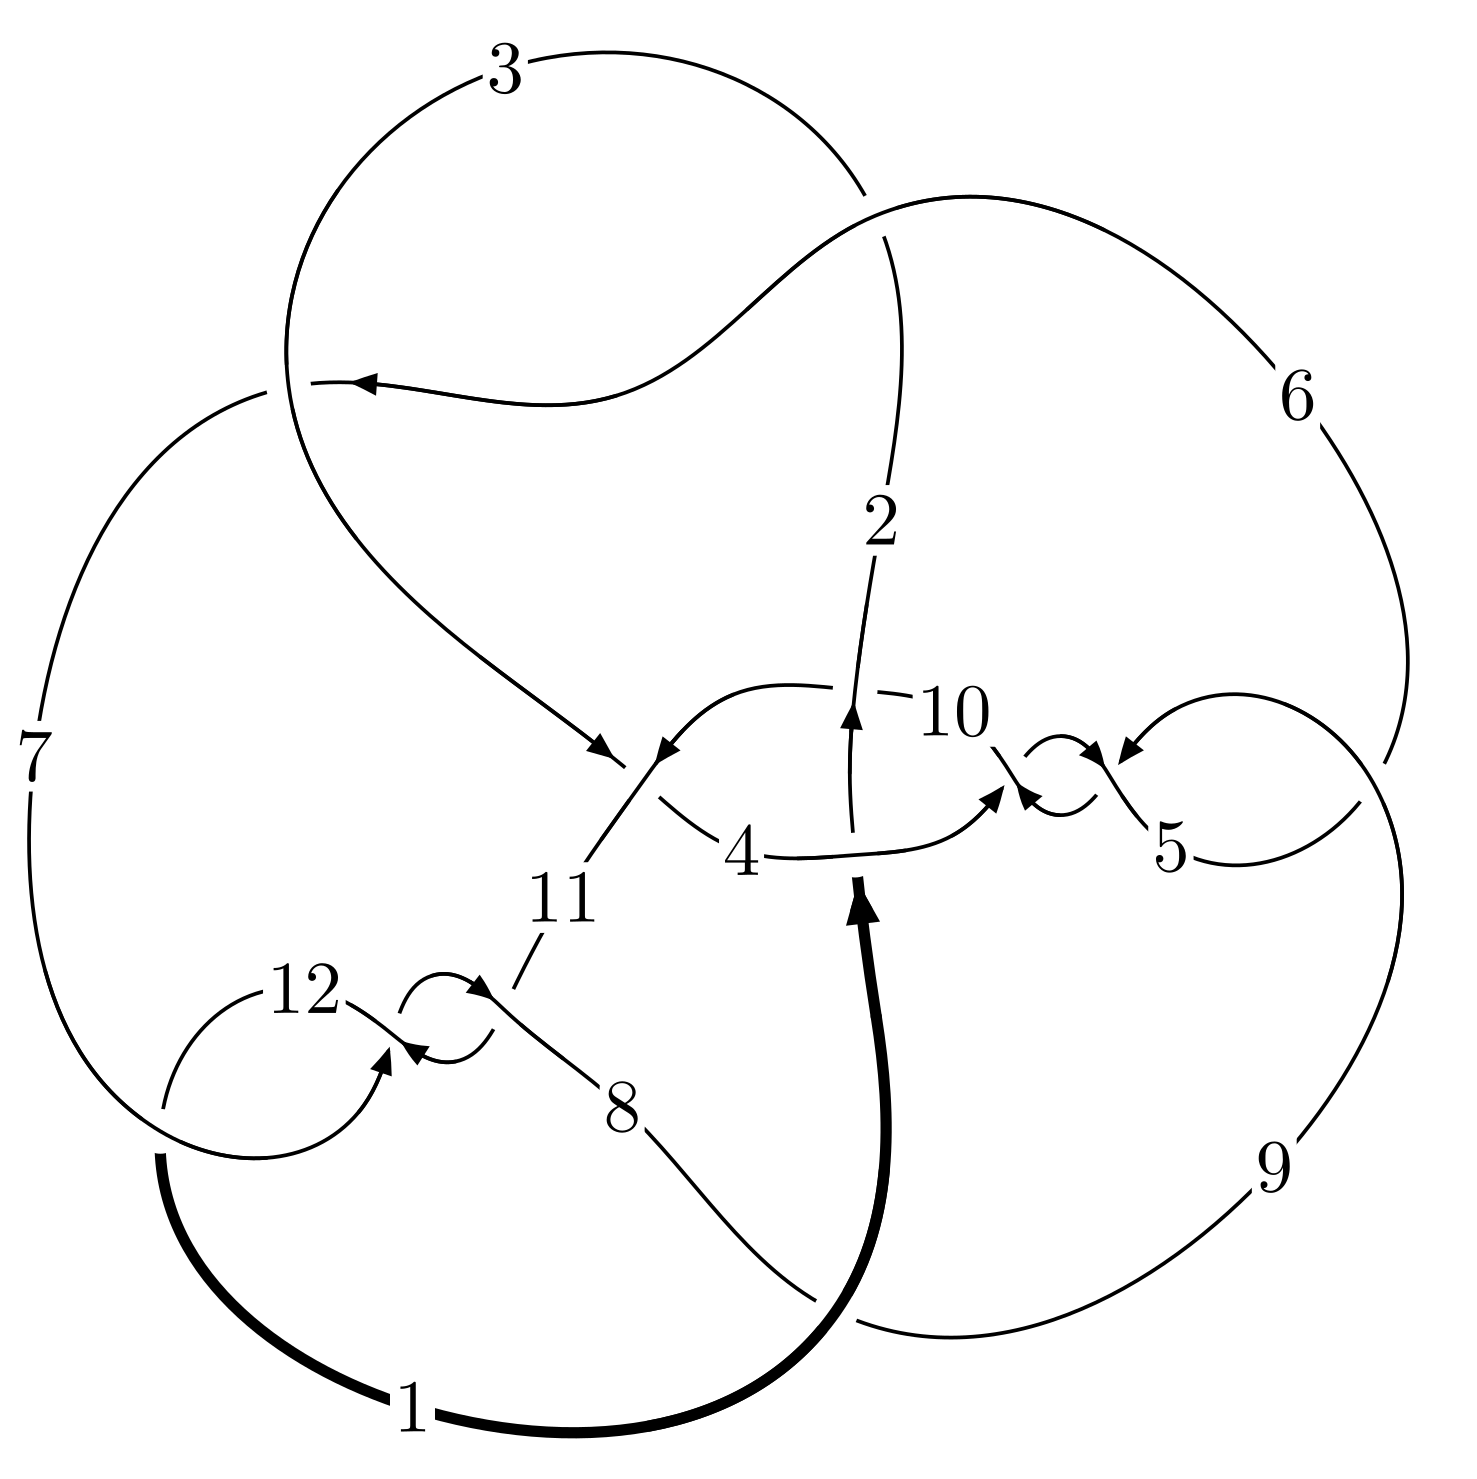
\includegraphics[width=112pt]{../../../GIT/diagram.site/Diagrams/png/1790_12a_0989.png}\\
\ \ \ A knot diagram\footnotemark}&
\allowdisplaybreaks
\textbf{Linearized knot diagam} \\
\cline{2-2}
 &
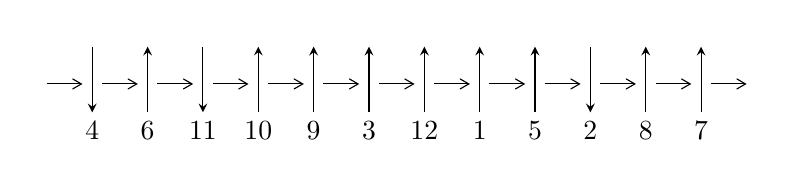
\begin{tikzpicture}[x=20pt, y=17pt]
	% nodes
	\node (C0) at (0, 0) {};
	\node (C1) at (1, 0) {};
	\node (C1U) at (1, +1) {};
	\node (C1D) at (1, -1) {4};

	\node (C2) at (2, 0) {};
	\node (C2U) at (2, +1) {};
	\node (C2D) at (2, -1) {6};

	\node (C3) at (3, 0) {};
	\node (C3U) at (3, +1) {};
	\node (C3D) at (3, -1) {11};

	\node (C4) at (4, 0) {};
	\node (C4U) at (4, +1) {};
	\node (C4D) at (4, -1) {10};

	\node (C5) at (5, 0) {};
	\node (C5U) at (5, +1) {};
	\node (C5D) at (5, -1) {9};

	\node (C6) at (6, 0) {};
	\node (C6U) at (6, +1) {};
	\node (C6D) at (6, -1) {3};

	\node (C7) at (7, 0) {};
	\node (C7U) at (7, +1) {};
	\node (C7D) at (7, -1) {12};

	\node (C8) at (8, 0) {};
	\node (C8U) at (8, +1) {};
	\node (C8D) at (8, -1) {1};

	\node (C9) at (9, 0) {};
	\node (C9U) at (9, +1) {};
	\node (C9D) at (9, -1) {5};

	\node (C10) at (10, 0) {};
	\node (C10U) at (10, +1) {};
	\node (C10D) at (10, -1) {2};

	\node (C11) at (11, 0) {};
	\node (C11U) at (11, +1) {};
	\node (C11D) at (11, -1) {8};

	\node (C12) at (12, 0) {};
	\node (C12U) at (12, +1) {};
	\node (C12D) at (12, -1) {7};
	\node (C13) at (13, 0) {};

	% arrows
	\draw[->,>={angle 60}]
	(C0) edge (C1) (C1) edge (C2) (C2) edge (C3) (C3) edge (C4) (C4) edge (C5) (C5) edge (C6) (C6) edge (C7) (C7) edge (C8) (C8) edge (C9) (C9) edge (C10) (C10) edge (C11) (C11) edge (C12) (C12) edge (C13) ;	\draw[->,>=stealth]
	(C1U) edge (C1D) (C2D) edge (C2U) (C3U) edge (C3D) (C4D) edge (C4U) (C5D) edge (C5U) (C6D) edge (C6U) (C7D) edge (C7U) (C8D) edge (C8U) (C9D) edge (C9U) (C10U) edge (C10D) (C11D) edge (C11U) (C12D) edge (C12U) ;
	\end{tikzpicture} \\
\hhline{~~} \\& 
\textbf{Solving Sequence} \\ \cline{2-2} 
 &
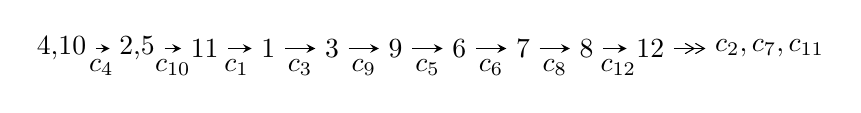
\begin{tikzpicture}[x=23pt, y=7pt]
	% node
	\node (A0) at (-1/8, 0) {4,10};
	\node (A1) at (17/16, 0) {2,5};
	\node (A2) at (17/8, 0) {11};
	\node (A3) at (25/8, 0) {1};
	\node (A4) at (33/8, 0) {3};
	\node (A5) at (41/8, 0) {9};
	\node (A6) at (49/8, 0) {6};
	\node (A7) at (57/8, 0) {7};
	\node (A8) at (65/8, 0) {8};
	\node (A9) at (73/8, 0) {12};
	\node (C1) at (1/2, -1) {$c_{4}$};
	\node (C2) at (13/8, -1) {$c_{10}$};
	\node (C3) at (21/8, -1) {$c_{1}$};
	\node (C4) at (29/8, -1) {$c_{3}$};
	\node (C5) at (37/8, -1) {$c_{9}$};
	\node (C6) at (45/8, -1) {$c_{5}$};
	\node (C7) at (53/8, -1) {$c_{6}$};
	\node (C8) at (61/8, -1) {$c_{8}$};
	\node (C9) at (69/8, -1) {$c_{12}$};
	\node (A10) at (11, 0) {$c_{2},c_{7},c_{11}$};

	% edge
	\draw[->,>=stealth]	
	(A0) edge (A1) (A1) edge (A2) (A2) edge (A3) (A3) edge (A4) (A4) edge (A5) (A5) edge (A6) (A6) edge (A7) (A7) edge (A8) (A8) edge (A9) ;
	\draw[->>,>={angle 60}]	
	(A9) edge (A10);
\end{tikzpicture} \\ 

\end{tabular} \\

\footnotetext{
The image of knot diagram is generated by the software ``\textbf{Draw programme}" developed by Andrew Bartholomew(\url{http://www.layer8.co.uk/maths/draw/index.htm\#Running-draw}), where we modified some parts for our purpose(\url{https://github.com/CATsTAILs/LinksPainter}).
}\phantom \\ \newline 
\centering \textbf{Ideals for irreducible components\footnotemark of $X_{\text{par}}$} 
 
\begin{align*}
I^u_{1}&=\langle 
2.17644\times10^{158} u^{92}-4.89354\times10^{158} u^{91}+\cdots+2.36703\times10^{158} b+2.64156\times10^{160},\\
\phantom{I^u_{1}}&\phantom{= \langle  }-1.71815\times10^{160} u^{92}+2.80396\times10^{160} u^{91}+\cdots+7.33779\times10^{159} a-2.19928\times10^{162},\\
\phantom{I^u_{1}}&\phantom{= \langle  }u^{93}-2 u^{92}+\cdots+272 u-31\rangle \\
I^u_{2}&=\langle 
u^{20}- u^{19}+\cdots+2 u^2+b,\;u^{17}- u^{16}+\cdots+a+4,\;u^{21}- u^{20}+\cdots+9 u^2+1\rangle \\
I^u_{3}&=\langle 
u^2+b,\;a-1,\;u^{15}+3 u^{13}- u^{10}-5 u^9-2 u^8+u^6+3 u^5+2 u^4- u^3- u^2+1\rangle \\
\\
\end{align*}
\raggedright * 3 irreducible components of $\dim_{\mathbb{C}}=0$, with total 129 representations.\\
\footnotetext{All coefficients of polynomials are rational numbers. But the coefficients are sometimes approximated in decimal forms when there is not enough margin.}
\newpage
\renewcommand{\arraystretch}{1}
\centering \section*{I. $I^u_{1}= \langle 2.18\times10^{158} u^{92}-4.89\times10^{158} u^{91}+\cdots+2.37\times10^{158} b+2.64\times10^{160},\;-1.72\times10^{160} u^{92}+2.80\times10^{160} u^{91}+\cdots+7.34\times10^{159} a-2.20\times10^{162},\;u^{93}-2 u^{92}+\cdots+272 u-31 \rangle$}
\flushleft \textbf{(i) Arc colorings}\\
\begin{tabular}{m{7pt} m{180pt} m{7pt} m{180pt} }
\flushright $a_{4}=$&$\begin{pmatrix}1\\0\end{pmatrix}$ \\
\flushright $a_{10}=$&$\begin{pmatrix}0\\u\end{pmatrix}$ \\
\flushright $a_{2}=$&$\begin{pmatrix}2.34150 u^{92}-3.82126 u^{91}+\cdots-1537.23 u+299.720\\-0.919480 u^{92}+2.06737 u^{91}+\cdots+662.190 u-111.598\end{pmatrix}$ \\
\flushright $a_{5}=$&$\begin{pmatrix}1\\- u^2\end{pmatrix}$ \\
\flushright $a_{11}=$&$\begin{pmatrix}-1.05704 u^{92}+2.58553 u^{91}+\cdots+713.093 u-107.997\\-1.32311 u^{92}+2.32703 u^{91}+\cdots+778.565 u-142.988\end{pmatrix}$ \\
\flushright $a_{1}=$&$\begin{pmatrix}1.42202 u^{92}-1.75388 u^{91}+\cdots-875.044 u+188.122\\-0.919480 u^{92}+2.06737 u^{91}+\cdots+662.190 u-111.598\end{pmatrix}$ \\
\flushright $a_{3}=$&$\begin{pmatrix}1.34484 u^{92}-1.75442 u^{91}+\cdots-1040.40 u+221.242\\-0.842160 u^{92}+1.62410 u^{91}+\cdots+516.189 u-89.1519\end{pmatrix}$ \\
\flushright $a_{9}=$&$\begin{pmatrix}- u\\u^3+u\end{pmatrix}$ \\
\flushright $a_{6}=$&$\begin{pmatrix}u^2+1\\- u^4-2 u^2\end{pmatrix}$ \\
\flushright $a_{7}=$&$\begin{pmatrix}-3.75367 u^{92}+6.11615 u^{91}+\cdots+2424.00 u-448.315\\2.03760 u^{92}-3.19078 u^{91}+\cdots-1029.66 u+188.557\end{pmatrix}$ \\
\flushright $a_{8}=$&$\begin{pmatrix}-3.68763 u^{92}+5.77130 u^{91}+\cdots+2009.93 u-364.805\\0.312514 u^{92}-0.432786 u^{91}+\cdots-141.093 u+24.4478\end{pmatrix}$ \\
\flushright $a_{12}=$&$\begin{pmatrix}-2.67125 u^{92}+4.38356 u^{91}+\cdots+1306.55 u-207.373\\-2.16240 u^{92}+3.42633 u^{91}+\cdots+1506.82 u-289.648\end{pmatrix}$\\&\end{tabular}
\flushleft \textbf{(ii) Obstruction class $= -1$}\\~\\
\flushleft \textbf{(iii) Cusp Shapes $= -2.26141 u^{92}+4.72648 u^{91}+\cdots+1127.48 u-174.399$}\\~\\
\newpage\renewcommand{\arraystretch}{1}
\flushleft \textbf{(iv) u-Polynomials at the component}\newline \\
\begin{tabular}{m{50pt}|m{274pt}}
Crossings & \hspace{64pt}u-Polynomials at each crossing \\
\hline $$\begin{aligned}c_{1}\end{aligned}$$&$\begin{aligned}
&u^{93}-9 u^{92}+\cdots+5549 u-149
\end{aligned}$\\
\hline $$\begin{aligned}c_{2},c_{6}\end{aligned}$$&$\begin{aligned}
&u^{93}-4 u^{92}+\cdots-16486 u-5639
\end{aligned}$\\
\hline $$\begin{aligned}c_{3}\end{aligned}$$&$\begin{aligned}
&u^{93}+13 u^{91}+\cdots-23676 u-2809
\end{aligned}$\\
\hline $$\begin{aligned}c_{4},c_{5},c_{9}\end{aligned}$$&$\begin{aligned}
&u^{93}-2 u^{92}+\cdots+272 u-31
\end{aligned}$\\
\hline $$\begin{aligned}c_{7},c_{11},c_{12}\end{aligned}$$&$\begin{aligned}
&u^{93}+5 u^{92}+\cdots-230 u-28
\end{aligned}$\\
\hline $$\begin{aligned}c_{8}\end{aligned}$$&$\begin{aligned}
&u^{93}-5 u^{92}+\cdots-978070 u-166348
\end{aligned}$\\
\hline $$\begin{aligned}c_{10}\end{aligned}$$&$\begin{aligned}
&u^{93}+7 u^{92}+\cdots+3131 u-509
\end{aligned}$\\
\hline
\end{tabular}\\~\\
\newpage\renewcommand{\arraystretch}{1}
\flushleft \textbf{(v) Riley Polynomials at the component}\newline \\
\begin{tabular}{m{50pt}|m{274pt}}
Crossings & \hspace{64pt}Riley Polynomials at each crossing \\
\hline $$\begin{aligned}c_{1}\end{aligned}$$&$\begin{aligned}
&y^{93}-7 y^{92}+\cdots+30482673 y-22201
\end{aligned}$\\
\hline $$\begin{aligned}c_{2},c_{6}\end{aligned}$$&$\begin{aligned}
&y^{93}-56 y^{92}+\cdots+966106988 y-31798321
\end{aligned}$\\
\hline $$\begin{aligned}c_{3}\end{aligned}$$&$\begin{aligned}
&y^{93}+26 y^{92}+\cdots-221556894 y-7890481
\end{aligned}$\\
\hline $$\begin{aligned}c_{4},c_{5},c_{9}\end{aligned}$$&$\begin{aligned}
&y^{93}+98 y^{92}+\cdots+49928 y-961
\end{aligned}$\\
\hline $$\begin{aligned}c_{7},c_{11},c_{12}\end{aligned}$$&$\begin{aligned}
&y^{93}+81 y^{92}+\cdots+1660 y-784
\end{aligned}$\\
\hline $$\begin{aligned}c_{8}\end{aligned}$$&$\begin{aligned}
&y^{93}-27 y^{92}+\cdots+59397369308 y-27671657104
\end{aligned}$\\
\hline $$\begin{aligned}c_{10}\end{aligned}$$&$\begin{aligned}
&y^{93}-19 y^{92}+\cdots+11519509 y-259081
\end{aligned}$\\
\hline
\end{tabular}\\~\\
\newpage\flushleft \textbf{(vi) Complex Volumes and Cusp Shapes}
$$\begin{array}{c|c|c}  
\text{Solutions to }I^u_{1}& \I (\text{vol} + \sqrt{-1}CS) & \text{Cusp shape}\\
 \hline 
\begin{aligned}
u &= \phantom{-}0.913602 + 0.442628 I \\
a &= -0.457622 + 1.243410 I \\
b &= \phantom{-}1.058510 - 0.914805 I\end{aligned}
 & -0.09995 + 12.96690 I & \phantom{-0.000000 } 0 \\ \hline\begin{aligned}
u &= \phantom{-}0.913602 - 0.442628 I \\
a &= -0.457622 - 1.243410 I \\
b &= \phantom{-}1.058510 + 0.914805 I\end{aligned}
 & -0.09995 - 12.96690 I & \phantom{-0.000000 } 0 \\ \hline\begin{aligned}
u &= \phantom{-}0.477137 + 0.859449 I \\
a &= -1.021430 - 0.010347 I \\
b &= \phantom{-}0.468897 + 0.485013 I\end{aligned}
 & \phantom{-}1.63423 - 0.00473 I & \phantom{-0.000000 } 0 \\ \hline\begin{aligned}
u &= \phantom{-}0.477137 - 0.859449 I \\
a &= -1.021430 + 0.010347 I \\
b &= \phantom{-}0.468897 - 0.485013 I\end{aligned}
 & \phantom{-}1.63423 + 0.00473 I & \phantom{-0.000000 } 0 \\ \hline\begin{aligned}
u &= -0.935734 + 0.449982 I \\
a &= -0.416168 + 0.107447 I \\
b &= \phantom{-}0.705075 - 0.315756 I\end{aligned}
 & -3.85014 - 0.96568 I & \phantom{-0.000000 } 0 \\ \hline\begin{aligned}
u &= -0.935734 - 0.449982 I \\
a &= -0.416168 - 0.107447 I \\
b &= \phantom{-}0.705075 + 0.315756 I\end{aligned}
 & -3.85014 + 0.96568 I & \phantom{-0.000000 } 0 \\ \hline\begin{aligned}
u &= -0.863338 + 0.408854 I \\
a &= -0.46911 - 1.34477 I \\
b &= \phantom{-}0.955959 + 0.919498 I\end{aligned}
 & \phantom{-}5.07812 - 8.87462 I & \phantom{-0.000000 } 0 \\ \hline\begin{aligned}
u &= -0.863338 - 0.408854 I \\
a &= -0.46911 + 1.34477 I \\
b &= \phantom{-}0.955959 - 0.919498 I\end{aligned}
 & \phantom{-}5.07812 + 8.87462 I & \phantom{-0.000000 } 0 \\ \hline\begin{aligned}
u &= -0.645207 + 0.651632 I \\
a &= \phantom{-}0.186968 - 1.274370 I \\
b &= \phantom{-}0.891416 + 0.487223 I\end{aligned}
 & -4.79645 - 4.22664 I & \phantom{-0.000000 } 0 \\ \hline\begin{aligned}
u &= -0.645207 - 0.651632 I \\
a &= \phantom{-}0.186968 + 1.274370 I \\
b &= \phantom{-}0.891416 - 0.487223 I\end{aligned}
 & -4.79645 + 4.22664 I & \phantom{-0.000000 } 0\\
 \hline 
 \end{array}$$\newpage$$\begin{array}{c|c|c}  
\text{Solutions to }I^u_{1}& \I (\text{vol} + \sqrt{-1}CS) & \text{Cusp shape}\\
 \hline 
\begin{aligned}
u &= -0.735166 + 0.839615 I \\
a &= -0.777511 - 0.042973 I \\
b &= \phantom{-}0.659808 - 0.589993 I\end{aligned}
 & \phantom{-}3.87469 + 3.43543 I & \phantom{-0.000000 } 0 \\ \hline\begin{aligned}
u &= -0.735166 - 0.839615 I \\
a &= -0.777511 + 0.042973 I \\
b &= \phantom{-}0.659808 + 0.589993 I\end{aligned}
 & \phantom{-}3.87469 - 3.43543 I & \phantom{-0.000000 } 0 \\ \hline\begin{aligned}
u &= \phantom{-}0.764831 + 0.380631 I \\
a &= -0.43381 + 1.55356 I \\
b &= \phantom{-}0.799947 - 0.860704 I\end{aligned}
 & \phantom{-}2.91231 + 4.47308 I & \phantom{-0.000000 } 0 \\ \hline\begin{aligned}
u &= \phantom{-}0.764831 - 0.380631 I \\
a &= -0.43381 - 1.55356 I \\
b &= \phantom{-}0.799947 + 0.860704 I\end{aligned}
 & \phantom{-}2.91231 - 4.47308 I & \phantom{-0.000000 } 0 \\ \hline\begin{aligned}
u &= \phantom{-}0.832710 + 0.861085 I \\
a &= -0.709125 + 0.097582 I \\
b &= \phantom{-}0.751222 + 0.616665 I\end{aligned}
 & -1.21449 - 7.09054 I & \phantom{-0.000000 } 0 \\ \hline\begin{aligned}
u &= \phantom{-}0.832710 - 0.861085 I \\
a &= -0.709125 - 0.097582 I \\
b &= \phantom{-}0.751222 - 0.616665 I\end{aligned}
 & -1.21449 + 7.09054 I & \phantom{-0.000000 } 0 \\ \hline\begin{aligned}
u &= -0.599446 + 0.529611 I \\
a &= \phantom{-}0.200504 + 1.259710 I \\
b &= -1.03242 - 1.03698 I\end{aligned}
 & -3.75102 - 7.23646 I & \phantom{-0.000000 } 0 \\ \hline\begin{aligned}
u &= -0.599446 - 0.529611 I \\
a &= \phantom{-}0.200504 - 1.259710 I \\
b &= -1.03242 + 1.03698 I\end{aligned}
 & -3.75102 + 7.23646 I & \phantom{-0.000000 } 0 \\ \hline\begin{aligned}
u &= \phantom{-}0.530203 + 0.536247 I \\
a &= -0.848529 - 0.391549 I \\
b &= \phantom{-}0.635048 + 0.428441 I\end{aligned}
 & \phantom{-}1.89674 - 0.16432 I & \phantom{-0.000000 } 0 \\ \hline\begin{aligned}
u &= \phantom{-}0.530203 - 0.536247 I \\
a &= -0.848529 + 0.391549 I \\
b &= \phantom{-}0.635048 - 0.428441 I\end{aligned}
 & \phantom{-}1.89674 + 0.16432 I & \phantom{-0.000000 } 0\\
 \hline 
 \end{array}$$\newpage$$\begin{array}{c|c|c}  
\text{Solutions to }I^u_{1}& \I (\text{vol} + \sqrt{-1}CS) & \text{Cusp shape}\\
 \hline 
\begin{aligned}
u &= \phantom{-}0.583719 + 0.435352 I \\
a &= \phantom{-}0.274470 - 1.263930 I \\
b &= -0.824406 + 0.986343 I\end{aligned}
 & \phantom{-}0.96715 + 3.76112 I & \phantom{-}6.00000 - 7.79854 I \\ \hline\begin{aligned}
u &= \phantom{-}0.583719 - 0.435352 I \\
a &= \phantom{-}0.274470 + 1.263930 I \\
b &= -0.824406 - 0.986343 I\end{aligned}
 & \phantom{-}0.96715 - 3.76112 I & \phantom{-}6.00000 + 7.79854 I \\ \hline\begin{aligned}
u &= \phantom{-}0.043409 + 1.292040 I \\
a &= -0.129329 + 1.260720 I \\
b &= -0.577513 - 1.162990 I\end{aligned}
 & -4.13101 - 4.56307 I & \phantom{-0.000000 } 0 \\ \hline\begin{aligned}
u &= \phantom{-}0.043409 - 1.292040 I \\
a &= -0.129329 - 1.260720 I \\
b &= -0.577513 + 1.162990 I\end{aligned}
 & -4.13101 + 4.56307 I & \phantom{-0.000000 } 0 \\ \hline\begin{aligned}
u &= -0.063260 + 1.309100 I \\
a &= -1.91793 - 0.51884 I \\
b &= -0.266745 - 0.059748 I\end{aligned}
 & \phantom{-}0.82618 - 2.85276 I & \phantom{-0.000000 } 0 \\ \hline\begin{aligned}
u &= -0.063260 - 1.309100 I \\
a &= -1.91793 + 0.51884 I \\
b &= -0.266745 + 0.059748 I\end{aligned}
 & \phantom{-}0.82618 + 2.85276 I & \phantom{-0.000000 } 0 \\ \hline\begin{aligned}
u &= -0.625101 + 0.280638 I \\
a &= \phantom{-}0.312212 + 1.130920 I \\
b &= -0.345387 - 1.035540 I\end{aligned}
 & -1.92190 - 0.78399 I & \phantom{-}6.00000 + 4.34634 I \\ \hline\begin{aligned}
u &= -0.625101 - 0.280638 I \\
a &= \phantom{-}0.312212 - 1.130920 I \\
b &= -0.345387 + 1.035540 I\end{aligned}
 & -1.92190 + 0.78399 I & \phantom{-}6.00000 - 4.34634 I \\ \hline\begin{aligned}
u &= \phantom{-}0.151548 + 1.312570 I \\
a &= -0.154828 - 0.278383 I \\
b &= \phantom{-}0.47612 + 2.10791 I\end{aligned}
 & -3.57737 + 7.92014 I & \phantom{-0.000000 } 0 \\ \hline\begin{aligned}
u &= \phantom{-}0.151548 - 1.312570 I \\
a &= -0.154828 + 0.278383 I \\
b &= \phantom{-}0.47612 - 2.10791 I\end{aligned}
 & -3.57737 - 7.92014 I & \phantom{-0.000000 } 0\\
 \hline 
 \end{array}$$\newpage$$\begin{array}{c|c|c}  
\text{Solutions to }I^u_{1}& \I (\text{vol} + \sqrt{-1}CS) & \text{Cusp shape}\\
 \hline 
\begin{aligned}
u &= -0.122631 + 1.319250 I \\
a &= -0.098610 + 0.261745 I \\
b &= \phantom{-}0.81321 - 1.84355 I\end{aligned}
 & \phantom{-}0.68667 - 3.90580 I & \phantom{-0.000000 } 0 \\ \hline\begin{aligned}
u &= -0.122631 - 1.319250 I \\
a &= -0.098610 - 0.261745 I \\
b &= \phantom{-}0.81321 + 1.84355 I\end{aligned}
 & \phantom{-}0.68667 + 3.90580 I & \phantom{-0.000000 } 0 \\ \hline\begin{aligned}
u &= \phantom{-}0.086300 + 1.323190 I \\
a &= -0.033382 - 0.229889 I \\
b &= \phantom{-}1.17676 + 1.47463 I\end{aligned}
 & -2.79990 - 0.13216 I & \phantom{-0.000000 } 0 \\ \hline\begin{aligned}
u &= \phantom{-}0.086300 - 1.323190 I \\
a &= -0.033382 + 0.229889 I \\
b &= \phantom{-}1.17676 - 1.47463 I\end{aligned}
 & -2.79990 + 0.13216 I & \phantom{-0.000000 } 0 \\ \hline\begin{aligned}
u &= -0.102451 + 1.339250 I \\
a &= \phantom{-}0.10172 - 1.45870 I \\
b &= -0.122372 + 1.064720 I\end{aligned}
 & \phantom{-}0.261156 - 0.373382 I & \phantom{-0.000000 } 0 \\ \hline\begin{aligned}
u &= -0.102451 - 1.339250 I \\
a &= \phantom{-}0.10172 + 1.45870 I \\
b &= -0.122372 - 1.064720 I\end{aligned}
 & \phantom{-}0.261156 + 0.373382 I & \phantom{-0.000000 } 0 \\ \hline\begin{aligned}
u &= \phantom{-}0.380036 + 1.300450 I \\
a &= -0.056447 - 0.899311 I \\
b &= -1.277570 + 0.597971 I\end{aligned}
 & -6.84431 + 2.10476 I & \phantom{-0.000000 } 0 \\ \hline\begin{aligned}
u &= \phantom{-}0.380036 - 1.300450 I \\
a &= -0.056447 + 0.899311 I \\
b &= -1.277570 - 0.597971 I\end{aligned}
 & -6.84431 - 2.10476 I & \phantom{-0.000000 } 0 \\ \hline\begin{aligned}
u &= \phantom{-}0.108724 + 1.377210 I \\
a &= -1.45681 + 0.90106 I \\
b &= -0.484326 + 0.094880 I\end{aligned}
 & -5.29511 + 7.48084 I & \phantom{-0.000000 } 0 \\ \hline\begin{aligned}
u &= \phantom{-}0.108724 - 1.377210 I \\
a &= -1.45681 - 0.90106 I \\
b &= -0.484326 - 0.094880 I\end{aligned}
 & -5.29511 - 7.48084 I & \phantom{-0.000000 } 0\\
 \hline 
 \end{array}$$\newpage$$\begin{array}{c|c|c}  
\text{Solutions to }I^u_{1}& \I (\text{vol} + \sqrt{-1}CS) & \text{Cusp shape}\\
 \hline 
\begin{aligned}
u &= \phantom{-}0.601998\phantom{ +0.000000I} \\
a &= \phantom{-}0.475355\phantom{ +0.000000I} \\
b &= \phantom{-}0.0274806\phantom{ +0.000000I}\end{aligned}
 & \phantom{-}0.846249\phantom{ +0.000000I} & \phantom{-}13.8440\phantom{ +0.000000I} \\ \hline\begin{aligned}
u &= \phantom{-}0.162275 + 1.400340 I \\
a &= \phantom{-}0.50117 + 1.37602 I \\
b &= \phantom{-}0.400795 - 0.971210 I\end{aligned}
 & -2.65152 + 5.81739 I & \phantom{-0.000000 } 0 \\ \hline\begin{aligned}
u &= \phantom{-}0.162275 - 1.400340 I \\
a &= \phantom{-}0.50117 - 1.37602 I \\
b &= \phantom{-}0.400795 + 0.971210 I\end{aligned}
 & -2.65152 - 5.81739 I & \phantom{-0.000000 } 0 \\ \hline\begin{aligned}
u &= \phantom{-}0.512131 + 0.278620 I \\
a &= -0.40132 + 2.59528 I \\
b &= \phantom{-}0.429005 - 0.669047 I\end{aligned}
 & \phantom{-}2.68816 + 3.40353 I & \phantom{-}11.5134 - 8.5198 I \\ \hline\begin{aligned}
u &= \phantom{-}0.512131 - 0.278620 I \\
a &= -0.40132 - 2.59528 I \\
b &= \phantom{-}0.429005 + 0.669047 I\end{aligned}
 & \phantom{-}2.68816 - 3.40353 I & \phantom{-}11.5134 + 8.5198 I \\ \hline\begin{aligned}
u &= -0.23586 + 1.39895 I \\
a &= -0.331701 + 0.594399 I \\
b &= -1.00644 - 1.34411 I\end{aligned}
 & -7.24895 - 3.91169 I & \phantom{-0.000000 } 0 \\ \hline\begin{aligned}
u &= -0.23586 - 1.39895 I \\
a &= -0.331701 - 0.594399 I \\
b &= -1.00644 + 1.34411 I\end{aligned}
 & -7.24895 + 3.91169 I & \phantom{-0.000000 } 0 \\ \hline\begin{aligned}
u &= -0.15703 + 1.42035 I \\
a &= -0.450171 + 0.829493 I \\
b &= -1.23858 - 0.89464 I\end{aligned}
 & -6.63384 - 3.20290 I & \phantom{-0.000000 } 0 \\ \hline\begin{aligned}
u &= -0.15703 - 1.42035 I \\
a &= -0.450171 - 0.829493 I \\
b &= -1.23858 + 0.89464 I\end{aligned}
 & -6.63384 + 3.20290 I & \phantom{-0.000000 } 0 \\ \hline\begin{aligned}
u &= \phantom{-}0.545802 + 0.030068 I \\
a &= \phantom{-}0.12360 - 1.47805 I \\
b &= \phantom{-}0.89653 + 1.26313 I\end{aligned}
 & \phantom{-}0.58881 + 5.47605 I & \phantom{-}10.85334 - 6.45978 I\\
 \hline 
 \end{array}$$\newpage$$\begin{array}{c|c|c}  
\text{Solutions to }I^u_{1}& \I (\text{vol} + \sqrt{-1}CS) & \text{Cusp shape}\\
 \hline 
\begin{aligned}
u &= \phantom{-}0.545802 - 0.030068 I \\
a &= \phantom{-}0.12360 + 1.47805 I \\
b &= \phantom{-}0.89653 - 1.26313 I\end{aligned}
 & \phantom{-}0.58881 - 5.47605 I & \phantom{-}10.85334 + 6.45978 I \\ \hline\begin{aligned}
u &= -0.39220 + 1.40768 I \\
a &= -0.005970 + 0.835212 I \\
b &= -1.127310 - 0.377774 I\end{aligned}
 & -3.51071 - 4.89100 I & \phantom{-0.000000 } 0 \\ \hline\begin{aligned}
u &= -0.39220 - 1.40768 I \\
a &= -0.005970 - 0.835212 I \\
b &= -1.127310 + 0.377774 I\end{aligned}
 & -3.51071 + 4.89100 I & \phantom{-0.000000 } 0 \\ \hline\begin{aligned}
u &= \phantom{-}0.24694 + 1.45463 I \\
a &= -0.035778 - 0.663022 I \\
b &= -0.542421 + 0.600773 I\end{aligned}
 & -4.63718 + 3.26112 I & \phantom{-0.000000 } 0 \\ \hline\begin{aligned}
u &= \phantom{-}0.24694 - 1.45463 I \\
a &= -0.035778 + 0.663022 I \\
b &= -0.542421 - 0.600773 I\end{aligned}
 & -4.63718 - 3.26112 I & \phantom{-0.000000 } 0 \\ \hline\begin{aligned}
u &= \phantom{-}0.21190 + 1.46415 I \\
a &= -0.502395 - 0.696276 I \\
b &= -1.45367 + 1.07755 I\end{aligned}
 & -5.16038 + 6.68364 I & \phantom{-0.000000 } 0 \\ \hline\begin{aligned}
u &= \phantom{-}0.21190 - 1.46415 I \\
a &= -0.502395 + 0.696276 I \\
b &= -1.45367 - 1.07755 I\end{aligned}
 & -5.16038 - 6.68364 I & \phantom{-0.000000 } 0 \\ \hline\begin{aligned}
u &= \phantom{-}0.203352 + 0.478894 I \\
a &= -0.15094 - 1.89057 I \\
b &= -1.154220 + 0.296388 I\end{aligned}
 & -6.65054 + 0.51603 I & -2.97629 - 0.81890 I \\ \hline\begin{aligned}
u &= \phantom{-}0.203352 - 0.478894 I \\
a &= -0.15094 + 1.89057 I \\
b &= -1.154220 - 0.296388 I\end{aligned}
 & -6.65054 - 0.51603 I & -2.97629 + 0.81890 I \\ \hline\begin{aligned}
u &= \phantom{-}0.09622 + 1.47913 I \\
a &= -0.610858 - 0.868754 I \\
b &= -1.33232 + 0.62691 I\end{aligned}
 & -13.10280 + 1.77082 I & \phantom{-0.000000 } 0\\
 \hline 
 \end{array}$$\newpage$$\begin{array}{c|c|c}  
\text{Solutions to }I^u_{1}& \I (\text{vol} + \sqrt{-1}CS) & \text{Cusp shape}\\
 \hline 
\begin{aligned}
u &= \phantom{-}0.09622 - 1.47913 I \\
a &= -0.610858 + 0.868754 I \\
b &= -1.33232 - 0.62691 I\end{aligned}
 & -13.10280 - 1.77082 I & \phantom{-0.000000 } 0 \\ \hline\begin{aligned}
u &= \phantom{-}0.17173 + 1.47790 I \\
a &= \phantom{-}0.338655 + 0.331113 I \\
b &= \phantom{-}0.899141 - 0.179238 I\end{aligned}
 & -4.77166 + 2.31742 I & \phantom{-0.000000 } 0 \\ \hline\begin{aligned}
u &= \phantom{-}0.17173 - 1.47790 I \\
a &= \phantom{-}0.338655 - 0.331113 I \\
b &= \phantom{-}0.899141 + 0.179238 I\end{aligned}
 & -4.77166 - 2.31742 I & \phantom{-0.000000 } 0 \\ \hline\begin{aligned}
u &= -0.04028 + 1.49084 I \\
a &= \phantom{-}0.263156 - 0.385197 I \\
b &= \phantom{-}0.762580 + 0.278955 I\end{aligned}
 & -4.89782 + 1.60324 I & \phantom{-0.000000 } 0 \\ \hline\begin{aligned}
u &= -0.04028 - 1.49084 I \\
a &= \phantom{-}0.263156 + 0.385197 I \\
b &= \phantom{-}0.762580 - 0.278955 I\end{aligned}
 & -4.89782 - 1.60324 I & \phantom{-0.000000 } 0 \\ \hline\begin{aligned}
u &= \phantom{-}0.28423 + 1.47284 I \\
a &= \phantom{-}0.539000 + 1.044640 I \\
b &= \phantom{-}1.09985 - 1.02283 I\end{aligned}
 & -3.07822 + 8.28484 I & \phantom{-0.000000 } 0 \\ \hline\begin{aligned}
u &= \phantom{-}0.28423 - 1.47284 I \\
a &= \phantom{-}0.539000 - 1.044640 I \\
b &= \phantom{-}1.09985 + 1.02283 I\end{aligned}
 & -3.07822 - 8.28484 I & \phantom{-0.000000 } 0 \\ \hline\begin{aligned}
u &= -0.395291 + 0.288983 I \\
a &= \phantom{-}0.71541 + 1.49210 I \\
b &= -0.674999 - 0.451166 I\end{aligned}
 & -1.12259 - 1.10724 I & -0.87157 + 3.08284 I \\ \hline\begin{aligned}
u &= -0.395291 - 0.288983 I \\
a &= \phantom{-}0.71541 - 1.49210 I \\
b &= -0.674999 + 0.451166 I\end{aligned}
 & -1.12259 + 1.10724 I & -0.87157 - 3.08284 I \\ \hline\begin{aligned}
u &= -0.21627 + 1.49749 I \\
a &= -0.555071 + 0.685058 I \\
b &= -1.60874 - 1.03760 I\end{aligned}
 & -10.3086 - 10.2526 I & \phantom{-0.000000 } 0\\
 \hline 
 \end{array}$$\newpage$$\begin{array}{c|c|c}  
\text{Solutions to }I^u_{1}& \I (\text{vol} + \sqrt{-1}CS) & \text{Cusp shape}\\
 \hline 
\begin{aligned}
u &= -0.21627 - 1.49749 I \\
a &= -0.555071 - 0.685058 I \\
b &= -1.60874 + 1.03760 I\end{aligned}
 & -10.3086 + 10.2526 I & \phantom{-0.000000 } 0 \\ \hline\begin{aligned}
u &= \phantom{-}0.42246 + 1.46495 I \\
a &= \phantom{-}0.038625 - 0.826763 I \\
b &= -1.119850 + 0.181789 I\end{aligned}
 & -8.15205 + 8.05269 I & \phantom{-0.000000 } 0 \\ \hline\begin{aligned}
u &= \phantom{-}0.42246 - 1.46495 I \\
a &= \phantom{-}0.038625 + 0.826763 I \\
b &= -1.119850 - 0.181789 I\end{aligned}
 & -8.15205 - 8.05269 I & \phantom{-0.000000 } 0 \\ \hline\begin{aligned}
u &= -0.32088 + 1.49052 I \\
a &= \phantom{-}0.518975 - 1.006450 I \\
b &= \phantom{-}1.27865 + 1.03826 I\end{aligned}
 & -1.03771 - 13.15390 I & \phantom{-0.000000 } 0 \\ \hline\begin{aligned}
u &= -0.32088 - 1.49052 I \\
a &= \phantom{-}0.518975 + 1.006450 I \\
b &= \phantom{-}1.27865 - 1.03826 I\end{aligned}
 & -1.03771 + 13.15390 I & \phantom{-0.000000 } 0 \\ \hline\begin{aligned}
u &= -0.20586 + 1.53058 I \\
a &= \phantom{-}0.701032 - 0.996276 I \\
b &= \phantom{-}0.961366 + 0.620833 I\end{aligned}
 & -11.88910 - 7.29226 I & \phantom{-0.000000 } 0 \\ \hline\begin{aligned}
u &= -0.20586 - 1.53058 I \\
a &= \phantom{-}0.701032 + 0.996276 I \\
b &= \phantom{-}0.961366 - 0.620833 I\end{aligned}
 & -11.88910 + 7.29226 I & \phantom{-0.000000 } 0 \\ \hline\begin{aligned}
u &= -0.449276 + 0.042466 I \\
a &= -0.03422 + 1.73671 I \\
b &= \phantom{-}1.07255 - 1.01805 I\end{aligned}
 & \phantom{-}4.94301 - 1.86722 I & \phantom{-}17.1351 + 4.2480 I \\ \hline\begin{aligned}
u &= -0.449276 - 0.042466 I \\
a &= -0.03422 - 1.73671 I \\
b &= \phantom{-}1.07255 + 1.01805 I\end{aligned}
 & \phantom{-}4.94301 + 1.86722 I & \phantom{-}17.1351 - 4.2480 I \\ \hline\begin{aligned}
u &= \phantom{-}0.33771 + 1.51180 I \\
a &= \phantom{-}0.515098 + 0.984249 I \\
b &= \phantom{-}1.38685 - 0.99515 I\end{aligned}
 & -6.3932 + 17.4899 I & \phantom{-0.000000 } 0\\
 \hline 
 \end{array}$$\newpage$$\begin{array}{c|c|c}  
\text{Solutions to }I^u_{1}& \I (\text{vol} + \sqrt{-1}CS) & \text{Cusp shape}\\
 \hline 
\begin{aligned}
u &= \phantom{-}0.33771 - 1.51180 I \\
a &= \phantom{-}0.515098 - 0.984249 I \\
b &= \phantom{-}1.38685 + 0.99515 I\end{aligned}
 & -6.3932 - 17.4899 I & \phantom{-0.000000 } 0 \\ \hline\begin{aligned}
u &= -0.27620 + 1.54799 I \\
a &= \phantom{-}0.075848 + 0.702148 I \\
b &= -0.489239 - 0.122470 I\end{aligned}
 & -9.41833 - 1.36160 I & \phantom{-0.000000 } 0 \\ \hline\begin{aligned}
u &= -0.27620 - 1.54799 I \\
a &= \phantom{-}0.075848 - 0.702148 I \\
b &= -0.489239 + 0.122470 I\end{aligned}
 & -9.41833 + 1.36160 I & \phantom{-0.000000 } 0 \\ \hline\begin{aligned}
u &= \phantom{-}0.00946 + 1.58941 I \\
a &= \phantom{-}0.299789 + 0.498833 I \\
b &= \phantom{-}0.636869 - 0.079459 I\end{aligned}
 & -10.78520 - 4.40021 I & \phantom{-0.000000 } 0 \\ \hline\begin{aligned}
u &= \phantom{-}0.00946 - 1.58941 I \\
a &= \phantom{-}0.299789 - 0.498833 I \\
b &= \phantom{-}0.636869 + 0.079459 I\end{aligned}
 & -10.78520 + 4.40021 I & \phantom{-0.000000 } 0 \\ \hline\begin{aligned}
u &= -0.24751 + 1.57309 I \\
a &= \phantom{-}0.359834 - 0.311803 I \\
b &= \phantom{-}0.910200 + 0.119775 I\end{aligned}
 & -10.91280 - 5.38166 I & \phantom{-0.000000 } 0 \\ \hline\begin{aligned}
u &= -0.24751 - 1.57309 I \\
a &= \phantom{-}0.359834 + 0.311803 I \\
b &= \phantom{-}0.910200 - 0.119775 I\end{aligned}
 & -10.91280 + 5.38166 I & \phantom{-0.000000 } 0 \\ \hline\begin{aligned}
u &= -0.390226 + 0.057007 I \\
a &= -2.61524 - 3.45928 I \\
b &= -0.001314 + 0.642526 I\end{aligned}
 & \phantom{-}4.67448 + 1.36905 I & \phantom{-}20.6717 - 3.3521 I \\ \hline\begin{aligned}
u &= -0.390226 - 0.057007 I \\
a &= -2.61524 + 3.45928 I \\
b &= -0.001314 - 0.642526 I\end{aligned}
 & \phantom{-}4.67448 - 1.36905 I & \phantom{-}20.6717 + 3.3521 I \\ \hline\begin{aligned}
u &= \phantom{-}0.346986 + 0.103915 I \\
a &= -4.06340 - 1.50940 I \\
b &= -0.345849 + 0.679582 I\end{aligned}
 & -0.47838 + 5.84762 I & \phantom{-}9.7633 - 10.6724 I\\
 \hline 
 \end{array}$$\newpage$$\begin{array}{c|c|c}  
\text{Solutions to }I^u_{1}& \I (\text{vol} + \sqrt{-1}CS) & \text{Cusp shape}\\
 \hline 
\begin{aligned}
u &= \phantom{-}0.346986 - 0.103915 I \\
a &= -4.06340 + 1.50940 I \\
b &= -0.345849 - 0.679582 I\end{aligned}
 & -0.47838 - 5.84762 I & \phantom{-}9.7633 + 10.6724 I \\ \hline\begin{aligned}
u &= \phantom{-}0.294798 + 0.013504 I \\
a &= -0.08216 - 2.66607 I \\
b &= \phantom{-}1.38561 + 0.72652 I\end{aligned}
 & \phantom{-}1.49403 - 1.59244 I & \phantom{-}14.2016 + 0.3191 I \\ \hline\begin{aligned}
u &= \phantom{-}0.294798 - 0.013504 I \\
a &= -0.08216 + 2.66607 I \\
b &= \phantom{-}1.38561 - 0.72652 I\end{aligned}
 & \phantom{-}1.49403 + 1.59244 I & \phantom{-}14.2016 - 0.3191 I\\
 \hline 
 \end{array}$$\newpage\newpage\renewcommand{\arraystretch}{1}
\centering \section*{II. $I^u_{2}= \langle u^{20}- u^{19}+\cdots+2 u^2+b,\;u^{17}- u^{16}+\cdots+a+4,\;u^{21}- u^{20}+\cdots+9 u^2+1 \rangle$}
\flushleft \textbf{(i) Arc colorings}\\
\begin{tabular}{m{7pt} m{180pt} m{7pt} m{180pt} }
\flushright $a_{4}=$&$\begin{pmatrix}1\\0\end{pmatrix}$ \\
\flushright $a_{10}=$&$\begin{pmatrix}0\\u\end{pmatrix}$ \\
\flushright $a_{2}=$&$\begin{pmatrix}- u^{17}+u^{16}+\cdots-16 u^2-4\\- u^{20}+u^{19}+\cdots- u^3-2 u^2\end{pmatrix}$ \\
\flushright $a_{5}=$&$\begin{pmatrix}1\\- u^2\end{pmatrix}$ \\
\flushright $a_{11}=$&$\begin{pmatrix}-4 u^{20}+4 u^{19}+\cdots-2 u^2-10 u\\- u^{19}+u^{18}+\cdots+2 u-1\end{pmatrix}$ \\
\flushright $a_{1}=$&$\begin{pmatrix}- u^{20}+u^{19}+\cdots-18 u^2-4\\- u^{20}+u^{19}+\cdots- u^3-2 u^2\end{pmatrix}$ \\
\flushright $a_{3}=$&$\begin{pmatrix}- u^{17}+u^{16}+\cdots-16 u^2-3\\u^{18}- u^{17}+\cdots-4 u^2+u\end{pmatrix}$ \\
\flushright $a_{9}=$&$\begin{pmatrix}- u\\u^3+u\end{pmatrix}$ \\
\flushright $a_{6}=$&$\begin{pmatrix}u^2+1\\- u^4-2 u^2\end{pmatrix}$ \\
\flushright $a_{7}=$&$\begin{pmatrix}- u^{20}+2 u^{19}+\cdots- u+5\\-4 u^{20}+4 u^{19}+\cdots+2 u^2-5 u\end{pmatrix}$ \\
\flushright $a_{8}=$&$\begin{pmatrix}u^{20}-5 u^{19}+\cdots-3 u-1\\u^{20}-4 u^{19}+\cdots-4 u^2+3 u\end{pmatrix}$ \\
\flushright $a_{12}=$&$\begin{pmatrix}-7 u^{20}+3 u^{19}+\cdots-7 u-6\\- u^{20}-4 u^{19}+\cdots+4 u-7\end{pmatrix}$\\&\end{tabular}
\flushleft \textbf{(ii) Obstruction class $= 1$}\\~\\
\flushleft \textbf{(iii) Cusp Shapes $= -4 u^{20}- u^{19}-34 u^{18}-17 u^{17}-105 u^{16}-93 u^{15}-108 u^{14}-232 u^{13}+112 u^{12}-261 u^{11}+327 u^{10}-64 u^9+134 u^8+75 u^7-201 u^6-10 u^5-205 u^4-47 u^3-60 u^2-3 u-2$}\\~\\
\newpage\renewcommand{\arraystretch}{1}
\flushleft \textbf{(iv) u-Polynomials at the component}\newline \\
\begin{tabular}{m{50pt}|m{274pt}}
Crossings & \hspace{64pt}u-Polynomials at each crossing \\
\hline $$\begin{aligned}c_{1}\end{aligned}$$&$\begin{aligned}
&u^{21}-4 u^{19}+\cdots+3 u-1
\end{aligned}$\\
\hline $$\begin{aligned}c_{2}\end{aligned}$$&$\begin{aligned}
&u^{21}-3 u^{20}+\cdots-9 u^2+1
\end{aligned}$\\
\hline $$\begin{aligned}c_{3}\end{aligned}$$&$\begin{aligned}
&u^{21}- u^{20}+\cdots+4 u^3+1
\end{aligned}$\\
\hline $$\begin{aligned}c_{4},c_{5}\end{aligned}$$&$\begin{aligned}
&u^{21}- u^{20}+\cdots+9 u^2+1
\end{aligned}$\\
\hline $$\begin{aligned}c_{6}\end{aligned}$$&$\begin{aligned}
&u^{21}+3 u^{20}+\cdots+9 u^2-1
\end{aligned}$\\
\hline $$\begin{aligned}c_{7}\end{aligned}$$&$\begin{aligned}
&u^{21}- u^{20}+\cdots-5 u^2+1
\end{aligned}$\\
\hline $$\begin{aligned}c_{8}\end{aligned}$$&$\begin{aligned}
&u^{21}+u^{20}+\cdots+2 u+1
\end{aligned}$\\
\hline $$\begin{aligned}c_{9}\end{aligned}$$&$\begin{aligned}
&u^{21}+u^{20}+\cdots-9 u^2-1
\end{aligned}$\\
\hline $$\begin{aligned}c_{10}\end{aligned}$$&$\begin{aligned}
&u^{21}-4 u^{18}+\cdots- u-1
\end{aligned}$\\
\hline $$\begin{aligned}c_{11},c_{12}\end{aligned}$$&$\begin{aligned}
&u^{21}+u^{20}+\cdots+5 u^2-1
\end{aligned}$\\
\hline
\end{tabular}\\~\\
\newpage\renewcommand{\arraystretch}{1}
\flushleft \textbf{(v) Riley Polynomials at the component}\newline \\
\begin{tabular}{m{50pt}|m{274pt}}
Crossings & \hspace{64pt}Riley Polynomials at each crossing \\
\hline $$\begin{aligned}c_{1}\end{aligned}$$&$\begin{aligned}
&y^{21}-8 y^{20}+\cdots+3 y-1
\end{aligned}$\\
\hline $$\begin{aligned}c_{2},c_{6}\end{aligned}$$&$\begin{aligned}
&y^{21}-21 y^{20}+\cdots+18 y-1
\end{aligned}$\\
\hline $$\begin{aligned}c_{3}\end{aligned}$$&$\begin{aligned}
&y^{21}-3 y^{20}+\cdots-8 y^2-1
\end{aligned}$\\
\hline $$\begin{aligned}c_{4},c_{5},c_{9}\end{aligned}$$&$\begin{aligned}
&y^{21}+21 y^{20}+\cdots-18 y-1
\end{aligned}$\\
\hline $$\begin{aligned}c_{7},c_{11},c_{12}\end{aligned}$$&$\begin{aligned}
&y^{21}+21 y^{20}+\cdots+10 y-1
\end{aligned}$\\
\hline $$\begin{aligned}c_{8}\end{aligned}$$&$\begin{aligned}
&y^{21}-7 y^{20}+\cdots+10 y-1
\end{aligned}$\\
\hline $$\begin{aligned}c_{10}\end{aligned}$$&$\begin{aligned}
&y^{21}+8 y^{19}+\cdots+3 y-1
\end{aligned}$\\
\hline
\end{tabular}\\~\\
\newpage\flushleft \textbf{(vi) Complex Volumes and Cusp Shapes}
$$\begin{array}{c|c|c}  
\text{Solutions to }I^u_{2}& \I (\text{vol} + \sqrt{-1}CS) & \text{Cusp shape}\\
 \hline 
\begin{aligned}
u &= \phantom{-}0.942504 + 0.246260 I \\
a &= \phantom{-}0.631734 - 0.286008 I \\
b &= -0.752858 - 0.134198 I\end{aligned}
 & -4.31301 + 1.48475 I & -2.43515 - 3.09049 I \\ \hline\begin{aligned}
u &= \phantom{-}0.942504 - 0.246260 I \\
a &= \phantom{-}0.631734 + 0.286008 I \\
b &= -0.752858 + 0.134198 I\end{aligned}
 & -4.31301 - 1.48475 I & -2.43515 + 3.09049 I \\ \hline\begin{aligned}
u &= -0.867402\phantom{ +0.000000I} \\
a &= \phantom{-}0.846213\phantom{ +0.000000I} \\
b &= -0.674358\phantom{ +0.000000I}\end{aligned}
 & \phantom{-}0.209182\phantom{ +0.000000I} & -3.13540\phantom{ +0.000000I} \\ \hline\begin{aligned}
u &= -0.024819 + 1.260640 I \\
a &= \phantom{-}0.873577 + 0.193046 I \\
b &= \phantom{-}1.79051 - 0.60013 I\end{aligned}
 & -1.87183 + 1.42542 I & \phantom{-}6.45818 - 0.53250 I \\ \hline\begin{aligned}
u &= -0.024819 - 1.260640 I \\
a &= \phantom{-}0.873577 - 0.193046 I \\
b &= \phantom{-}1.79051 + 0.60013 I\end{aligned}
 & -1.87183 - 1.42542 I & \phantom{-}6.45818 + 0.53250 I \\ \hline\begin{aligned}
u &= \phantom{-}0.051916 + 1.310110 I \\
a &= \phantom{-}1.134780 - 0.699911 I \\
b &= \phantom{-}0.761655 + 0.696872 I\end{aligned}
 & \phantom{-}0.60500 + 2.12401 I & \phantom{-}7.45502 - 0.61311 I \\ \hline\begin{aligned}
u &= \phantom{-}0.051916 - 1.310110 I \\
a &= \phantom{-}1.134780 + 0.699911 I \\
b &= \phantom{-}0.761655 - 0.696872 I\end{aligned}
 & \phantom{-}0.60500 - 2.12401 I & \phantom{-}7.45502 + 0.61311 I \\ \hline\begin{aligned}
u &= -0.116459 + 1.317440 I \\
a &= \phantom{-}0.529330 + 0.945267 I \\
b &= \phantom{-}0.127554 - 1.169550 I\end{aligned}
 & -4.23054 - 6.68298 I & \phantom{-}3.09112 + 5.24011 I \\ \hline\begin{aligned}
u &= -0.116459 - 1.317440 I \\
a &= \phantom{-}0.529330 - 0.945267 I \\
b &= \phantom{-}0.127554 + 1.169550 I\end{aligned}
 & -4.23054 + 6.68298 I & \phantom{-}3.09112 - 5.24011 I \\ \hline\begin{aligned}
u &= \phantom{-}0.315230 + 1.339510 I \\
a &= -0.047136 - 0.641467 I \\
b &= -1.16096 + 0.82040 I\end{aligned}
 & -8.03930 + 2.94569 I & -3.03387 - 2.74900 I\\
 \hline 
 \end{array}$$\newpage$$\begin{array}{c|c|c}  
\text{Solutions to }I^u_{2}& \I (\text{vol} + \sqrt{-1}CS) & \text{Cusp shape}\\
 \hline 
\begin{aligned}
u &= \phantom{-}0.315230 - 1.339510 I \\
a &= -0.047136 + 0.641467 I \\
b &= -1.16096 - 0.82040 I\end{aligned}
 & -8.03930 - 2.94569 I & -3.03387 + 2.74900 I \\ \hline\begin{aligned}
u &= -0.313919 + 0.482198 I \\
a &= -0.35009 + 1.42347 I \\
b &= -0.070636 + 0.740220 I\end{aligned}
 & -1.00960 + 5.13706 I & \phantom{-}3.81791 - 2.57618 I \\ \hline\begin{aligned}
u &= -0.313919 - 0.482198 I \\
a &= -0.35009 - 1.42347 I \\
b &= -0.070636 - 0.740220 I\end{aligned}
 & -1.00960 - 5.13706 I & \phantom{-}3.81791 + 2.57618 I \\ \hline\begin{aligned}
u &= -0.077295 + 0.557233 I \\
a &= -1.226070 + 0.444963 I \\
b &= \phantom{-}0.974734 + 0.496814 I\end{aligned}
 & \phantom{-}0.81376 - 1.77615 I & \phantom{-}1.80485 + 4.14303 I \\ \hline\begin{aligned}
u &= -0.077295 - 0.557233 I \\
a &= -1.226070 - 0.444963 I \\
b &= \phantom{-}0.974734 - 0.496814 I\end{aligned}
 & \phantom{-}0.81376 + 1.77615 I & \phantom{-}1.80485 - 4.14303 I \\ \hline\begin{aligned}
u &= -0.27572 + 1.43267 I \\
a &= -0.199332 + 0.719503 I \\
b &= -0.867664 - 0.619835 I\end{aligned}
 & -4.77951 - 4.11317 I & \phantom{-}3.13796 + 6.16435 I \\ \hline\begin{aligned}
u &= -0.27572 - 1.43267 I \\
a &= -0.199332 - 0.719503 I \\
b &= -0.867664 + 0.619835 I\end{aligned}
 & -4.77951 + 4.11317 I & \phantom{-}3.13796 - 6.16435 I \\ \hline\begin{aligned}
u &= \phantom{-}0.162734 + 0.459737 I \\
a &= -1.36050 - 1.34511 I \\
b &= \phantom{-}0.361068 - 0.517119 I\end{aligned}
 & \phantom{-}3.85234 - 1.38121 I & \phantom{-}8.78785 + 1.62457 I \\ \hline\begin{aligned}
u &= \phantom{-}0.162734 - 0.459737 I \\
a &= -1.36050 + 1.34511 I \\
b &= \phantom{-}0.361068 + 0.517119 I\end{aligned}
 & \phantom{-}3.85234 + 1.38121 I & \phantom{-}8.78785 - 1.62457 I \\ \hline\begin{aligned}
u &= \phantom{-}0.26953 + 1.56759 I \\
a &= -0.409400 - 0.556126 I \\
b &= -0.826230 + 0.337958 I\end{aligned}
 & -10.74070 + 6.05778 I & \phantom{-}1.98382 - 7.58727 I\\
 \hline 
 \end{array}$$\newpage$$\begin{array}{c|c|c}  
\text{Solutions to }I^u_{2}& \I (\text{vol} + \sqrt{-1}CS) & \text{Cusp shape}\\
 \hline 
\begin{aligned}
u &= \phantom{-}0.26953 - 1.56759 I \\
a &= -0.409400 + 0.556126 I \\
b &= -0.826230 - 0.337958 I\end{aligned}
 & -10.74070 - 6.05778 I & \phantom{-}1.98382 + 7.58727 I\\
 \hline 
 \end{array}$$\newpage\newpage\renewcommand{\arraystretch}{1}
\centering \section*{III. $I^u_{3}= \langle u^2+b,\;a-1,\;u^{15}+3 u^{13}+\cdots- u^2+1 \rangle$}
\flushleft \textbf{(i) Arc colorings}\\
\begin{tabular}{m{7pt} m{180pt} m{7pt} m{180pt} }
\flushright $a_{4}=$&$\begin{pmatrix}1\\0\end{pmatrix}$ \\
\flushright $a_{10}=$&$\begin{pmatrix}0\\u\end{pmatrix}$ \\
\flushright $a_{2}=$&$\begin{pmatrix}1\\- u^2\end{pmatrix}$ \\
\flushright $a_{5}=$&$\begin{pmatrix}1\\- u^2\end{pmatrix}$ \\
\flushright $a_{11}=$&$\begin{pmatrix}- u\\u^3+u\end{pmatrix}$ \\
\flushright $a_{1}=$&$\begin{pmatrix}- u^2+1\\- u^2\end{pmatrix}$ \\
\flushright $a_{3}=$&$\begin{pmatrix}u^4+u^2+1\\- u^6-2 u^4- u^2\end{pmatrix}$ \\
\flushright $a_{9}=$&$\begin{pmatrix}- u\\u^3+u\end{pmatrix}$ \\
\flushright $a_{6}=$&$\begin{pmatrix}u^2+1\\- u^4-2 u^2\end{pmatrix}$ \\
\flushright $a_{7}=$&$\begin{pmatrix}- u^6- u^4+1\\u^8+2 u^6-2 u^2\end{pmatrix}$ \\
\flushright $a_{8}=$&$\begin{pmatrix}- u^7+2 u^3-2 u\\- u^7- u^5+2 u^3+u\end{pmatrix}$ \\
\flushright $a_{12}=$&$\begin{pmatrix}u^{12}+u^{11}+u^{10}+2 u^9-3 u^8- u^7- u^6-2 u^5+3 u^4+u^3-2 u^2- u+1\\- u^{13}+u^{12}-3 u^{11}+2 u^{10}- u^9- u^8+3 u^7-2 u^6+u^5+u^4- u^2+u\end{pmatrix}$\\&\end{tabular}
\flushleft \textbf{(ii) Obstruction class $= -1$}\\~\\
\flushleft \textbf{(iii) Cusp Shapes $= -4 u^5-4 u^3+4 u+6$}\\~\\
\newpage\renewcommand{\arraystretch}{1}
\flushleft \textbf{(iv) u-Polynomials at the component}\newline \\
\begin{tabular}{m{50pt}|m{274pt}}
Crossings & \hspace{64pt}u-Polynomials at each crossing \\
\hline $$\begin{aligned}c_{1}\end{aligned}$$&$\begin{aligned}
&u^{15}-6 u^{14}+\cdots+2 u+1
\end{aligned}$\\
\hline $$\begin{aligned}c_{2},c_{6}\end{aligned}$$&$\begin{aligned}
&u^{15}+6 u^{14}+\cdots+2 u-1
\end{aligned}$\\
\hline $$\begin{aligned}c_{3}\end{aligned}$$&$\begin{aligned}
&u^{15}-3 u^{13}+\cdots+4 u+5
\end{aligned}$\\
\hline $$\begin{aligned}c_{4},c_{5},c_{9}\\c_{10}\end{aligned}$$&$\begin{aligned}
&u^{15}+3 u^{13}- u^{10}-5 u^9-2 u^8+u^6+3 u^5+2 u^4- u^3- u^2+1
\end{aligned}$\\
\hline $$\begin{aligned}c_{7},c_{11},c_{12}\end{aligned}$$&$\begin{aligned}
&(u^3- u^2+2 u-1)^5
\end{aligned}$\\
\hline $$\begin{aligned}c_{8}\end{aligned}$$&$\begin{aligned}
&(u^3+u^2-1)^5
\end{aligned}$\\
\hline
\end{tabular}\\~\\
\newpage\renewcommand{\arraystretch}{1}
\flushleft \textbf{(v) Riley Polynomials at the component}\newline \\
\begin{tabular}{m{50pt}|m{274pt}}
Crossings & \hspace{64pt}Riley Polynomials at each crossing \\
\hline $$\begin{aligned}c_{1},c_{2},c_{6}\end{aligned}$$&$\begin{aligned}
&y^{15}-18 y^{14}+\cdots-6 y-1
\end{aligned}$\\
\hline $$\begin{aligned}c_{3}\end{aligned}$$&$\begin{aligned}
&y^{15}-6 y^{14}+\cdots-134 y-25
\end{aligned}$\\
\hline $$\begin{aligned}c_{4},c_{5},c_{9}\\c_{10}\end{aligned}$$&$\begin{aligned}
&y^{15}+6 y^{14}+\cdots+2 y-1
\end{aligned}$\\
\hline $$\begin{aligned}c_{7},c_{11},c_{12}\end{aligned}$$&$\begin{aligned}
&(y^3+3 y^2+2 y-1)^5
\end{aligned}$\\
\hline $$\begin{aligned}c_{8}\end{aligned}$$&$\begin{aligned}
&(y^3- y^2+2 y-1)^5
\end{aligned}$\\
\hline
\end{tabular}\\~\\
\newpage\flushleft \textbf{(vi) Complex Volumes and Cusp Shapes}
$$\begin{array}{c|c|c}  
\text{Solutions to }I^u_{3}& \I (\text{vol} + \sqrt{-1}CS) & \text{Cusp shape}\\
 \hline 
\begin{aligned}
u &= \phantom{-}1.003770 + 0.106833 I \\
a &= \phantom{-}1.00000\phantom{ +0.000000I} \\
b &= -0.996143 - 0.214471 I\end{aligned}
 & -3.02413 + 2.82812 I & \phantom{-}2.49024 - 2.97945 I \\ \hline\begin{aligned}
u &= \phantom{-}1.003770 - 0.106833 I \\
a &= \phantom{-}1.00000\phantom{ +0.000000I} \\
b &= -0.996143 + 0.214471 I\end{aligned}
 & -3.02413 - 2.82812 I & \phantom{-}2.49024 + 2.97945 I \\ \hline\begin{aligned}
u &= -0.962445\phantom{ +0.000000I} \\
a &= \phantom{-}1.00000\phantom{ +0.000000I} \\
b &= -0.926301\phantom{ +0.000000I}\end{aligned}
 & \phantom{-}1.11345\phantom{ +0.000000I} & \phantom{-}9.01950\phantom{ +0.000000I} \\ \hline\begin{aligned}
u &= -0.803235 + 0.362184 I \\
a &= \phantom{-}1.00000\phantom{ +0.000000I} \\
b &= -0.514010 + 0.581838 I\end{aligned}
 & -3.02413 + 2.82812 I & \phantom{-}2.49024 - 2.97945 I \\ \hline\begin{aligned}
u &= -0.803235 - 0.362184 I \\
a &= \phantom{-}1.00000\phantom{ +0.000000I} \\
b &= -0.514010 - 0.581838 I\end{aligned}
 & -3.02413 - 2.82812 I & \phantom{-}2.49024 + 2.97945 I \\ \hline\begin{aligned}
u &= \phantom{-}0.168874 + 1.219270 I \\
a &= \phantom{-}1.00000\phantom{ +0.000000I} \\
b &= \phantom{-}1.45811 - 0.41181 I\end{aligned}
 & -3.02413 - 2.82812 I & \phantom{-}2.49024 + 2.97945 I \\ \hline\begin{aligned}
u &= \phantom{-}0.168874 - 1.219270 I \\
a &= \phantom{-}1.00000\phantom{ +0.000000I} \\
b &= \phantom{-}1.45811 + 0.41181 I\end{aligned}
 & -3.02413 + 2.82812 I & \phantom{-}2.49024 - 2.97945 I \\ \hline\begin{aligned}
u &= -0.450135 + 0.619793 I \\
a &= \phantom{-}1.00000\phantom{ +0.000000I} \\
b &= \phantom{-}0.181522 + 0.557981 I\end{aligned}
 & -3.02413 - 2.82812 I & \phantom{-}2.49024 + 2.97945 I \\ \hline\begin{aligned}
u &= -0.450135 - 0.619793 I \\
a &= \phantom{-}1.00000\phantom{ +0.000000I} \\
b &= \phantom{-}0.181522 - 0.557981 I\end{aligned}
 & -3.02413 + 2.82812 I & \phantom{-}2.49024 - 2.97945 I \\ \hline\begin{aligned}
u &= -0.096333 + 1.293630 I \\
a &= \phantom{-}1.00000\phantom{ +0.000000I} \\
b &= \phantom{-}1.66419 + 0.24924 I\end{aligned}
 & \phantom{-}1.11345\phantom{ +0.000000I} & \phantom{-}9.01951 + 0. I\phantom{ +0.000000I}\\
 \hline 
 \end{array}$$\newpage$$\begin{array}{c|c|c}  
\text{Solutions to }I^u_{3}& \I (\text{vol} + \sqrt{-1}CS) & \text{Cusp shape}\\
 \hline 
\begin{aligned}
u &= -0.096333 - 1.293630 I \\
a &= \phantom{-}1.00000\phantom{ +0.000000I} \\
b &= \phantom{-}1.66419 - 0.24924 I\end{aligned}
 & \phantom{-}1.11345\phantom{ +0.000000I} & \phantom{-}9.01951 + 0. I\phantom{ +0.000000I} \\ \hline\begin{aligned}
u &= \phantom{-}0.577555 + 0.364050 I \\
a &= \phantom{-}1.00000\phantom{ +0.000000I} \\
b &= -0.201038 - 0.420518 I\end{aligned}
 & \phantom{-}1.11345\phantom{ +0.000000I} & \phantom{-}9.01951 + 0. I\phantom{ +0.000000I} \\ \hline\begin{aligned}
u &= \phantom{-}0.577555 - 0.364050 I \\
a &= \phantom{-}1.00000\phantom{ +0.000000I} \\
b &= -0.201038 + 0.420518 I\end{aligned}
 & \phantom{-}1.11345\phantom{ +0.000000I} & \phantom{-}9.01951 + 0. I\phantom{ +0.000000I} \\ \hline\begin{aligned}
u &= \phantom{-}0.080725 + 1.370050 I \\
a &= \phantom{-}1.00000\phantom{ +0.000000I} \\
b &= \phantom{-}1.87052 - 0.22119 I\end{aligned}
 & -3.02413 + 2.82812 I & \phantom{-}2.49024 - 2.97945 I \\ \hline\begin{aligned}
u &= \phantom{-}0.080725 - 1.370050 I \\
a &= \phantom{-}1.00000\phantom{ +0.000000I} \\
b &= \phantom{-}1.87052 + 0.22119 I\end{aligned}
 & -3.02413 - 2.82812 I & \phantom{-}2.49024 + 2.97945 I\\
 \hline 
 \end{array}$$\newpage
\newpage\renewcommand{\arraystretch}{1}
\centering \section*{ IV. u-Polynomials}
\begin{tabular}{m{50pt}|m{274pt}}
Crossings & \hspace{64pt}u-Polynomials at each crossing \\
\hline $$\begin{aligned}c_{1}\end{aligned}$$&$\begin{aligned}
&(u^{15}-6 u^{14}+\cdots+2 u+1)(u^{21}-4 u^{19}+\cdots+3 u-1)\\
&\cdot(u^{93}-9 u^{92}+\cdots+5549 u-149)
\end{aligned}$\\
\hline $$\begin{aligned}c_{2}\end{aligned}$$&$\begin{aligned}
&(u^{15}+6 u^{14}+\cdots+2 u-1)(u^{21}-3 u^{20}+\cdots-9 u^2+1)\\
&\cdot(u^{93}-4 u^{92}+\cdots-16486 u-5639)
\end{aligned}$\\
\hline $$\begin{aligned}c_{3}\end{aligned}$$&$\begin{aligned}
&(u^{15}-3 u^{13}+\cdots+4 u+5)(u^{21}- u^{20}+\cdots+4 u^3+1)\\
&\cdot(u^{93}+13 u^{91}+\cdots-23676 u-2809)
\end{aligned}$\\
\hline $$\begin{aligned}c_{4},c_{5}\end{aligned}$$&$\begin{aligned}
&(u^{15}+3 u^{13}- u^{10}-5 u^9-2 u^8+u^6+3 u^5+2 u^4- u^3- u^2+1)\\
&\cdot(u^{21}- u^{20}+\cdots+9 u^2+1)(u^{93}-2 u^{92}+\cdots+272 u-31)
\end{aligned}$\\
\hline $$\begin{aligned}c_{6}\end{aligned}$$&$\begin{aligned}
&(u^{15}+6 u^{14}+\cdots+2 u-1)(u^{21}+3 u^{20}+\cdots+9 u^2-1)\\
&\cdot(u^{93}-4 u^{92}+\cdots-16486 u-5639)
\end{aligned}$\\
\hline $$\begin{aligned}c_{7}\end{aligned}$$&$\begin{aligned}
&((u^3- u^2+2 u-1)^5)(u^{21}- u^{20}+\cdots-5 u^2+1)\\
&\cdot(u^{93}+5 u^{92}+\cdots-230 u-28)
\end{aligned}$\\
\hline $$\begin{aligned}c_{8}\end{aligned}$$&$\begin{aligned}
&((u^3+u^2-1)^5)(u^{21}+u^{20}+\cdots+2 u+1)\\
&\cdot(u^{93}-5 u^{92}+\cdots-978070 u-166348)
\end{aligned}$\\
\hline $$\begin{aligned}c_{9}\end{aligned}$$&$\begin{aligned}
&(u^{15}+3 u^{13}- u^{10}-5 u^9-2 u^8+u^6+3 u^5+2 u^4- u^3- u^2+1)\\
&\cdot(u^{21}+u^{20}+\cdots-9 u^2-1)(u^{93}-2 u^{92}+\cdots+272 u-31)
\end{aligned}$\\
\hline $$\begin{aligned}c_{10}\end{aligned}$$&$\begin{aligned}
&(u^{15}+3 u^{13}- u^{10}-5 u^9-2 u^8+u^6+3 u^5+2 u^4- u^3- u^2+1)\\
&\cdot(u^{21}-4 u^{18}+\cdots- u-1)(u^{93}+7 u^{92}+\cdots+3131 u-509)
\end{aligned}$\\
\hline $$\begin{aligned}c_{11},c_{12}\end{aligned}$$&$\begin{aligned}
&((u^3- u^2+2 u-1)^5)(u^{21}+u^{20}+\cdots+5 u^2-1)\\
&\cdot(u^{93}+5 u^{92}+\cdots-230 u-28)
\end{aligned}$\\
\hline
\end{tabular}\newpage\renewcommand{\arraystretch}{1}
\centering \section*{ V. Riley Polynomials}
\begin{tabular}{m{50pt}|m{274pt}}
Crossings & \hspace{64pt}Riley Polynomials at each crossing \\
\hline $$\begin{aligned}c_{1}\end{aligned}$$&$\begin{aligned}
&(y^{15}-18 y^{14}+\cdots-6 y-1)(y^{21}-8 y^{20}+\cdots+3 y-1)\\
&\cdot(y^{93}-7 y^{92}+\cdots+30482673 y-22201)
\end{aligned}$\\
\hline $$\begin{aligned}c_{2},c_{6}\end{aligned}$$&$\begin{aligned}
&(y^{15}-18 y^{14}+\cdots-6 y-1)(y^{21}-21 y^{20}+\cdots+18 y-1)\\
&\cdot(y^{93}-56 y^{92}+\cdots+966106988 y-31798321)
\end{aligned}$\\
\hline $$\begin{aligned}c_{3}\end{aligned}$$&$\begin{aligned}
&(y^{15}-6 y^{14}+\cdots-134 y-25)(y^{21}-3 y^{20}+\cdots-8 y^2-1)\\
&\cdot(y^{93}+26 y^{92}+\cdots-221556894 y-7890481)
\end{aligned}$\\
\hline $$\begin{aligned}c_{4},c_{5},c_{9}\end{aligned}$$&$\begin{aligned}
&(y^{15}+6 y^{14}+\cdots+2 y-1)(y^{21}+21 y^{20}+\cdots-18 y-1)\\
&\cdot(y^{93}+98 y^{92}+\cdots+49928 y-961)
\end{aligned}$\\
\hline $$\begin{aligned}c_{7},c_{11},c_{12}\end{aligned}$$&$\begin{aligned}
&((y^3+3 y^2+2 y-1)^5)(y^{21}+21 y^{20}+\cdots+10 y-1)\\
&\cdot(y^{93}+81 y^{92}+\cdots+1660 y-784)
\end{aligned}$\\
\hline $$\begin{aligned}c_{8}\end{aligned}$$&$\begin{aligned}
&((y^3- y^2+2 y-1)^5)(y^{21}-7 y^{20}+\cdots+10 y-1)\\
&\cdot(y^{93}-27 y^{92}+\cdots+59397369308 y-27671657104)
\end{aligned}$\\
\hline $$\begin{aligned}c_{10}\end{aligned}$$&$\begin{aligned}
&(y^{15}+6 y^{14}+\cdots+2 y-1)(y^{21}+8 y^{19}+\cdots+3 y-1)\\
&\cdot(y^{93}-19 y^{92}+\cdots+11519509 y-259081)
\end{aligned}$\\
\hline
\end{tabular}
\vskip 2pc
\end{document}